\section{The immersed boundary method}\label{sec:ib}

\subsection{Overview}\label{sec:ib_old}

Consider a rectangular domain, $\domain\subset\R^3$, which contains one or more
deformable structures and is otherwise filled with an incompressible, Newtonian fluid
with constant density, $\density$, and viscosity, $\viscosity$. The IB method treats
these structures as an extension of the fluid. The motion of any particle in $\domain$ is
therefore governed by the incompressible Navier-Stokes equations,
\begin{gather}
    \density(\u_t + \div(\u\otimes\u)) = \viscosity\laplacian \u - \grad p + \f, \label{eq:ins-momentum} \\
    \div \u = 0, \label{eq:ins-incomp}
\end{gather}
where, for $\x = (x,\,y,\,z) \in \domain$, $\u = \u(\x,\,t) = (u, v, w)$ is the fluid
velocity, $p = p(\x,\,t)$ is the pressure, and $\f = \f(\x,\,t)$ is an external force
density. Here and throughout this paper, we use bold italic symbols to indicate a vector
in $\R^3$. Treating the entire domain as a fluid allows us to discretize $\domain$
independently of the immersed structures with a fixed regular grid of spacing $h$. This
is the Eulerian grid.

Let $\X = \X(\theta,\,\varphi,\,t)$, for surface coordinates $(\theta,\,\varphi)$ in
$\sites\subset\mathbb{R}^2$, be a parametrization for the immersed boundary $\interface$.
Though the interface changes with time, we suppress the time argument $t$ for brevity. A
discrete representation of the boundary, consisting of a set of surface points, replaces
its continuous counterpart.  Surface points are typically chosen to be within
approximately $h$ of their neighbors.  This is the Lagrangian grid. These boundary points
move at the local fluid velocity.  Analytically convolving the fluid velocity against the
Dirac delta function, $\Dirac(\x)$, yields the velocity of a surface point, but
discretely, Eulerian and Lagrangian grid points are unlikely to coincide. The IB method
replaces the singular Dirac delta function with a smoothed, $h$-dependent analog,
$\Dirac_h(\x)$. The Lagrangian point $\X$ evolves according to
\begin{equation}\label{eq:ib-interp}
    \vec{\dot{X}}
        = \int\limits_{\domain} \u(\x) \Dirac(\x-\X) \d\x
        \approx h^3 \sum_{i} \u(\x_i) \Dirac_h(\x_i-\X),
\end{equation}
where $i$ enumerates the Eulerian grid points, and a superposed dot denotes partial
differentiation with respect to $t$. As a boundary deforms, it generates a force density
$\F = \F(\X,\,t)$, which it imparts onto the fluid as $\f$ in~\eqref{eq:ins-momentum}.
Again, we suppress $t$ when using $\F$. By similar reasoning as the velocity, $\F$ is
transferred to the fluid at $\x$ via
\begin{equation}\label{eq:ib-spread}
        \f(\x)
        = \int\limits_{\interface} \F(\X)\Dirac(\x-\X) \d\X
        \approx \sum_{j} \weight[j]\F(\X_j) \Dirac_h(\x-\X_j),
\end{equation}
where $j$ enumerates the Lagrangian grid points, and $\weight[j]$ is the integration
weight corresponding to Lagrangian grid point $\X_j$. 

In addition to a velocity vector field, equation~\eqref{eq:ib-spread} illustrates the
need for three pieces of information for each immersed structure: the position of points
$\X_j$ used to evaluate forces on the structure; a force density $\F(\X_j)$ at each of
those points; and surface integration weights $\weight[j]$ for those points. The
structure moves according to~\eqref{eq:ib-interp}. The next three sections describe our
methods for solving~\eqref{eq:ins-momentum}--\eqref{eq:ins-incomp} (Section~%
\ref{sec:ins}), give analytic expressions for energy functionals used to derive $\F$
(Section~\ref{sec:energy} and~\ref{sec:forces}), and detail the discretization of the
structures to obtain $\X_j$, $\F(\X_j)$, and $\weight[j]$ (Section~\ref{sec:rbfs}).
However, before we do so, we discuss the specific variant of the IB method employed
herein.

\subsection{The RBF-IB method}\label{sec:rbfib}

The classical IB method uses the same the Lagrangian points in interpolation~%
\eqref{eq:ib-interp} and spreading~\eqref{eq:ib-spread}. However, there exist several IB
methods use different sets of points instead. For instance, the method in~%
\cite{Griffith:2017id} uses a finite element representation for the structure, and
consequently spreads forces from (Lagrangian) quadrature points, interpolates velocities
to quadrature points, and then projects them using the finite element basis to the
individual element nodes. The RBF-IB method introduced in~\cite{Shankar:2015km} and used
in this work also does something similar. A small set of $\data\cardinality$ Lagrangian
points approximately $2h$ apart is used to approximate $\X$ and this set of points is
moved by~\eqref{eq:ib-interp}. In addition, a larger set of $\sample\cardinality$ points
chosen to be approximately $h$ apart is used to spread forces using~\eqref{eq:ib-spread}.
While the former set is widely spaced, the spacing of the latter set of points aligns
with traditional IB implementations.

This potentially raises certain concerns, which we address here. The first major concern
relates to the force-spreading and velocity interpolation operations. In traditional IB
methods, these operators are formally adjoint, leading to conservation of energy/power~%
\cite{Peskin:2002go}. However, in the RBF-IB method, these operators are no longer
adjoint, leading to concerns about numerical stability. In previous work~%
\cite{Shankar:2015km}, the authors demonstrated that the RBF-IB method dissipated energy
in 2D simulations as expected, despite the absence of formal adjointness. In this work,
we show similar results for an RBC relaxation problem in a full 3D simulation in Section%
~\ref{sec:energy}. The second major concern related to the wide $2h$ spacing of the
smaller set of points used to approximate $\X$ and update the structure. If the points
are spaced too widely apart, it is possible to obtain unphysical behavior, with some
parts of the structure responding more to the neighboring fluid than others.  However,
both in~\cite{Shankar:2015km} and in this work, we observed that starting these points
with a spacing of $2h$ was sufficient to reproduce standard results for RBC simulations.
It may be possible to alleviate any spacing issues by periodically rearranging the points
used to approximate $\X$, but this approach was not necessary in this work, and so we
leave a full exploration of such Lagrangian rearrangement strategies for future work.

\section{Solution of the incompressible Navier-Stokes equations}\label{sec:ins}

\subsection{Spatial Discretization}\label{sec:ns_space}

To discretize the Navier-Stokes equations~\eqref{eq:ins-momentum} and~\eqref{eq:ins-incomp}, we use a
marker-and-cell (MAC) grid~\cite{Welch:1965jv}: for grid cell center $\x_i$, scalar-valued function $s(\x)$ is
discretized at $\x_i$, and component $\e_a\cdot\vec{v}$ of vector-valued function $\vec{v}(\x)$ at
$\x_i-\sfrac12h\e_a$, where $\e_a$ is a canonical basis vector. Define the centered difference operator
\begin{equation}
    D_a\phi(\x) = \frac{\phi(\x+\sfrac12 h\e_a) - \phi(\x-\sfrac12 h\e_a)}{h},
\end{equation}
for which, \latin{e.g.}, $D_1$ approximates differentiation in the $x$ direction. The discrete divergence,
gradient, and Laplacian operators use centered differences, resulting in a 2-point stencil for each discrete first
derivative and the standard 7-point discrete Laplacian. We also define the centered average operator
\begin{equation}
    A_a\phi(\x) = \frac{\phi(\x+\sfrac12 h\e_a) + \phi(\x-\sfrac12 h\e_a)}2.
\end{equation}
By averaging $u$ in the $y$ direction and $v$ in the $x$ direction, we obtain collocated approximations to $u$ and
$v$ at the center of a cell edge. Averaging, e.g., $u$ in the $x$ direction yields an approximation to $u$ at the
cell center. We can therefore discretize the components of the advection term $\div(\u\otimes\u)$ by
\begin{equation}\label{eq:advection}
    \div[h](\u\otimes\u) :=
    \begin{bmatrix}
        D_1[(A_1 u) (A_1 u)] + D_2[(A_1 v) (A_2 u)] + D_3[(A_1 w) (A_3 u)] \\
        D_1[(A_2 u) (A_1 v)] + D_2[(A_2 v) (A_2 v)] + D_3[(A_2 w) (A_3 v)] \\
        D_1[(A_3 u) (A_1 w)] + D_2[(A_3 v) (A_2 w)] + D_3[(A_3 w) (A_3 w)]
    \end{bmatrix}.
\end{equation}
The symbol $\div[h]$ represents the discrete divergence operator.  \Cref{fig:discretization} illustrates the steps
in computing $D_2[(A_1 v)(A_2 u)]$, which appears in the first component in~\eqref{eq:advection}. Morinishi
\latin{et al.}~\cite{Morinishi:1998us} show that this scheme, $Div. - S2$ in their parlance, is conservative under
the assumption that $\u$ is discretely divergence-free.

\begin{figure}[tb]
    \centering
    \begin{subfigure}{0.33\textwidth}
        \centering
    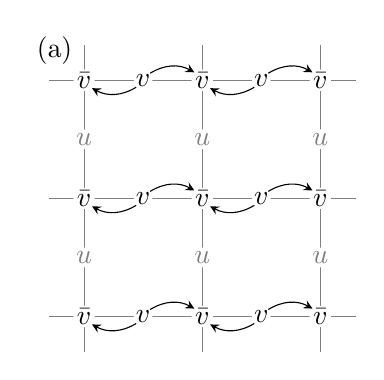
\begin{tikzpicture}[scale=1.5]
        \draw[help lines] (-0.3, -0.3) grid (2.3, 2.3);

        \foreach \x in {0,...,2}
            \foreach \y in {0,...,1}
            {
                \node[circle, inner sep=0pt, color=black!50, fill=white] at (\x, \y+0.5) {$u$};
            }
        \foreach \y in {0,...,2}
        {
            \foreach \x in {0,...,2}
                \node[circle, inner sep=0pt, fill=white] (av\x\y) at (\x, \y) {$\bar{v}$};
            \foreach \x in {0,...,1}
                \node[circle, inner sep=0pt, fill=white] (v\x\y) at (\x+0.5, \y) {$v$};
        }
        \path[-stealth] (v00.south west) edge[bend left] node[midway, below, yshift=+1pt] {} (av00.south east);
        \path[-stealth] (v10.south west) edge[bend left] node[midway, below, yshift=+1pt] {} (av10.south east);
        %\path[-stealth] (v20.south west) edge[bend left] node[midway, below, yshift=+1pt] {} (av20.south east);
        \path[-stealth] (v01.south west) edge[bend left] node[midway, below, yshift=+1pt] {} (av01.south east);
        \path[-stealth] (v11.south west) edge[bend left] node[midway, below, yshift=+1pt] {} (av11.south east);
        %\path[-stealth] (v21.south west) edge[bend left] node[midway, below, yshift=+1pt] {} (av21.south east);
        \path[-stealth] (v02.south west) edge[bend left] node[midway, below, yshift=+1pt] {} (av02.south east);
        \path[-stealth] (v12.south west) edge[bend left] node[midway, below, yshift=+1pt] {} (av12.south east);
        %\path[-stealth] (v22.south west) edge[bend left] node[midway, below, yshift=+1pt] {} (av22.south east);
        %\path[-stealth] (v03.south west) edge[bend left] node[midway, below, yshift=+1pt] {} (av03.south east);
        %\path[-stealth] (v13.south west) edge[bend left] node[midway, below, yshift=+1pt] {} (av13.south east);
        %\path[-stealth] (v23.south west) edge[bend left] node[midway, below, yshift=+1pt] {} (av23.south east);

        \path[-stealth] (v00.north east) edge[bend left] node[midway, below, yshift=+1pt] {} (av10.north west);
        \path[-stealth] (v10.north east) edge[bend left] node[midway, below, yshift=+1pt] {} (av20.north west);
        %\path[-stealth] (v20.north east) edge[bend left] node[midway, below, yshift=+1pt] {} (av30.north west);
        \path[-stealth] (v01.north east) edge[bend left] node[midway, below, yshift=+1pt] {} (av11.north west);
        \path[-stealth] (v11.north east) edge[bend left] node[midway, below, yshift=+1pt] {} (av21.north west);
        %\path[-stealth] (v21.north east) edge[bend left] node[midway, below, yshift=+1pt] {} (av31.north west);
        \path[-stealth] (v02.north east) edge[bend left] node[midway, below, yshift=+1pt] {} (av12.north west);
        \path[-stealth] (v12.north east) edge[bend left] node[midway, below, yshift=+1pt] {} (av22.north west);
        %\path[-stealth] (v22.north east) edge[bend left] node[midway, below, yshift=+1pt] {} (av32.north west);
        %\path[-stealth] (v03.north east) edge[bend left] node[midway, below, yshift=+1pt] {} (av13.north west);
        %\path[-stealth] (v13.north east) edge[bend left] node[midway, below, yshift=+1pt] {} (av23.north west);
        %\path[-stealth] (v23.north east) edge[bend left] node[midway, below, yshift=+1pt] {} (av33.north west);

        \node[black] at (-0.25, 2.25) {(a)};
    \end{tikzpicture}
    \label{fig:adv-x-ave}
    \end{subfigure}%
    \begin{subfigure}{0.33\textwidth}
        \centering
    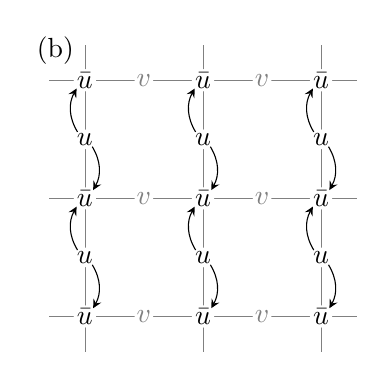
\begin{tikzpicture}[scale=1.5]
        \draw[help lines] (-0.3, -0.3) grid (2.3, 2.3);

        \foreach \x in {0,...,2}
        {
            \foreach \y in {0,...,1}
            {
                \node[circle, inner sep=0pt, fill=white] (u\x\y) at (\x, \y+0.5) {$u$};
            }
            \foreach \y in {0,...,2}
            {
                \node[circle, inner sep=0pt, fill=white] (au\x\y) at (\x, \y) {$\bar{u}$};
            }
        }
        \foreach \x in {0,...,1}
            \foreach \y in {0,...,2}
            {
                \node[circle, inner sep=0pt, color=black!50, fill=white] at (\x+0.5, \y) {$v$};
            }

        \path[-stealth] (u00.south east) edge[bend left] node[midway, below, yshift=+1pt] {} (au00.north east);
        \path[-stealth] (u10.south east) edge[bend left] node[midway, below, yshift=+1pt] {} (au10.north east);
        \path[-stealth] (u20.south east) edge[bend left] node[midway, below, yshift=+1pt] {} (au20.north east);
        %\path[-stealth] (u30.south east) edge[bend left] node[midway, below, yshift=+1pt] {} (au30.north east);
        \path[-stealth] (u01.south east) edge[bend left] node[midway, below, yshift=+1pt] {} (au01.north east);
        \path[-stealth] (u11.south east) edge[bend left] node[midway, below, yshift=+1pt] {} (au11.north east);
        \path[-stealth] (u21.south east) edge[bend left] node[midway, below, yshift=+1pt] {} (au21.north east);
        %\path[-stealth] (u31.south east) edge[bend left] node[midway, below, yshift=+1pt] {} (au31.north east);
        %\path[-stealth] (u02.south east) edge[bend left] node[midway, below, yshift=+1pt] {} (au02.north east);
        %\path[-stealth] (u12.south east) edge[bend left] node[midway, below, yshift=+1pt] {} (au12.north east);
        %\path[-stealth] (u22.south east) edge[bend left] node[midway, below, yshift=+1pt] {} (au22.north east);
        %\path[-stealth] (u32.south east) edge[bend left] node[midway, below, yshift=+1pt] {} (au32.north east);

        \path[-stealth] (u00.north west) edge[bend left] node[midway, below, yshift=+1pt] {} (au01.south west);
        \path[-stealth] (u10.north west) edge[bend left] node[midway, below, yshift=+1pt] {} (au11.south west);
        \path[-stealth] (u20.north west) edge[bend left] node[midway, below, yshift=+1pt] {} (au21.south west);
        %\path[-stealth] (u30.north west) edge[bend left] node[midway, below, yshift=+1pt] {} (au31.south west);
        \path[-stealth] (u01.north west) edge[bend left] node[midway, below, yshift=+1pt] {} (au02.south west);
        \path[-stealth] (u11.north west) edge[bend left] node[midway, below, yshift=+1pt] {} (au12.south west);
        \path[-stealth] (u21.north west) edge[bend left] node[midway, below, yshift=+1pt] {} (au22.south west);
        %\path[-stealth] (u31.north west) edge[bend left] node[midway, below, yshift=+1pt] {} (au32.south west);
        %\path[-stealth] (u02.north west) edge[bend left] node[midway, below, yshift=+1pt] {} (au03.south west);
        %\path[-stealth] (u12.north west) edge[bend left] node[midway, below, yshift=+1pt] {} (au13.south west);
        %\path[-stealth] (u22.north west) edge[bend left] node[midway, below, yshift=+1pt] {} (au23.south west);
        %\path[-stealth] (u32.north west) edge[bend left] node[midway, below, yshift=+1pt] {} (au33.south west);
        \node[black] at (-0.25, 2.25) {(b)};
    \end{tikzpicture}
    \label{fig:adv-y-ave}
    \end{subfigure}%
    \begin{subfigure}{0.33\textwidth}
        \centering
    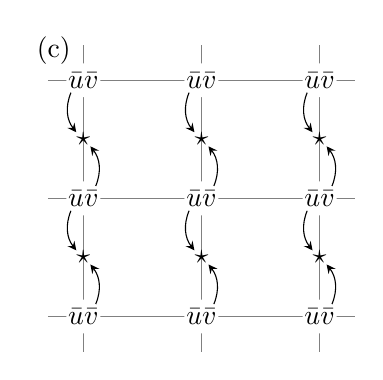
\begin{tikzpicture}[scale=1.5]
        \draw[help lines] (-0.3, -0.3) grid (2.3, 2.3);

        \foreach \x in {0,...,2}
            \foreach \y in {0,...,2}
                \node[circle, inner sep=0pt, fill=white] (uv\x\y) at (\x, \y) {$\bar{u}\bar{v}$};
        \foreach \x in {0,...,2}
            \foreach \y in {0,...,1}
                \node[circle, inner sep=0pt] (duv\x\y) at (\x, \y+0.5) {$\star$};

        \path[stealth-] (duv00.south east) edge[bend left] (uv00.north east);
        \path[stealth-] (duv10.south east) edge[bend left] (uv10.north east);
        \path[stealth-] (duv20.south east) edge[bend left] (uv20.north east);
        %\path[stealth-] (duv30.south east) edge[bend left] (uv30.north east);
        \path[stealth-] (duv01.south east) edge[bend left] (uv01.north east);
        \path[stealth-] (duv11.south east) edge[bend left] (uv11.north east);
        \path[stealth-] (duv21.south east) edge[bend left] (uv21.north east);
        %\path[stealth-] (duv31.south east) edge[bend left] (uv31.north east);
        %\path[stealth-] (duv02.south east) edge[bend left] (uv02.north east);
        %\path[stealth-] (duv12.south east) edge[bend left] (uv12.north east);
        %\path[stealth-] (duv22.south east) edge[bend left] (uv22.north east);
        %\path[stealth-] (duv32.south east) edge[bend left] (uv32.north east);

        \path[stealth-] (duv00.north west) edge[bend left] (uv01.south west);
        \path[stealth-] (duv10.north west) edge[bend left] (uv11.south west);
        \path[stealth-] (duv20.north west) edge[bend left] (uv21.south west);
        %\path[stealth-] (duv30.north west) edge[bend left] (uv31.south west);
        \path[stealth-] (duv01.north west) edge[bend left] (uv02.south west);
        \path[stealth-] (duv11.north west) edge[bend left] (uv12.south west);
        \path[stealth-] (duv21.north west) edge[bend left] (uv22.south west);
        %\path[stealth-] (duv31.north west) edge[bend left] (uv32.south west);
        %\path[stealth-] (duv02.north west) edge[bend left] (uv03.south west);
        %\path[stealth-] (duv12.north west) edge[bend left] (uv13.south west);
        %\path[stealth-] (duv22.north west) edge[bend left] (uv23.south west);
        %\path[stealth-] (duv32.north west) edge[bend left] (uv33.south west);
        \node[black] at (-0.25, 2.25) {(c)};
    \end{tikzpicture}
    \label{fig:adv-y-diff}
    \end{subfigure}%
    \caption{%
A cross-section illustrating the steps in computing the $D_2[(A_2 u) (A_1 v)]$ term of the first component of the
advection. The horizontal and vertical velocity component discretization locations are marked by $u$ and $v$,
respectively. Arrows emanate from a point contributing to a stencil and point to the center of the stencil.
(a) $A_1$ averages $v$ in the $x$ direction, yielding an approximation $\bar{v}$ at grid vertices (in 3D, centers
of cell edges for which $x$ and $y$ are constant).
(b) $A_2$ averages $u$ in the $y$ direction, yielding an approximation $\bar{u}$ at the same points as (a). The
quantities $A_1 v$ and $A_2 u$ are collocated and can be directly multiplied to obtain an approximation of $uv$ at
locations marked $\bar{u}\bar{v}$.
(c) $D_2$ approximately differentiates $uv$ in the $y$ direction, yielding the desired quantity at each point
marked $\star$.  The approximation of $uv$ is also used to compute $D_1[(A_1 v)(A_2 u)]$ in the second component
of the advection, wherein application of $D_1$ instead yields approximations collocated with locations marked $v$
in (a).
    }
    \label{fig:discretization}
\end{figure}


\subsection{Temporal Discretization}\label{sec:ns_time}

To advance the solution, we use either the backward-forward Euler-based scheme~\cite{Ascher:1997tm} or the 2-stage
scheme described by Peskin~\cite{Peskin:2002go}, modified to advance structures using the newest velocities. The
modification makes these schemes formally first-order in time, but allow us to separate the Eulerian update from
the Lagrangian update by requiring only information at the beginning of the timestep to evaluate forces and moving
the structure at the end of the timestep. For the backward-forward Euler scheme, discretizing~%
\eqref{eq:ins-momentum} to advance time to $t+\timestep$, yields linear solves of Helmholtz type,
\begin{equation}\label{eq:disc-momentum}
    (I - \timestep\rho^{-1}\mu \laplacian_h) \u^\ast = \u^n - \timestep\left[\div[h]\left(\u^n\otimes\u^n\right) + \rho^{-1}\left(\f^{n+1} - \grad[h]p^n\right)\right] \quad\text{in}~\domain, \\
\end{equation}
with boundary conditions
\begin{equation}\label{eq:disc-bdy}
    \u^\ast = \u^{n+1}_b + \timestep \grad[h] q^{n} \quad\text{on}~\partial\domain,
\end{equation}
where superscripts denote the time step, $\u_b$ is velocity boundary data, $\laplacian_h$ and $\grad[h]$ are the
discrete Laplacian and gradient, respectively, and $q$ is described below. The force density $\f^{n+1}$ is
advanced using only data at timestep $n$. The intermediate velocity field $\u^\ast$ may not be divergence-free. To
obtain a velocity field that satisfies~\eqref{eq:ins-incomp}, we use projection method II (PmII) of Brown, Cortez,
and Minion~\cite{Brown:2001bq}. PmII updates the pressure using
\begin{equation}
    p^{n+1} = p^n + (\rho I - \timestep\mu\laplacian_h)q^{n+1},
\end{equation}
and generates the divergence-free velocity field
\begin{equation}\label{eq:vel-update}
    \u^{n+1} = \u^\ast - \timestep\grad[h]q^{n+1}
\end{equation}
using the pseudo-pressure $q^{n+1}$, which satisfies
\begin{equation}
\begin{alignedat}{2}
    &k \laplacian_h q^{n+1} = \div[h]\u^\ast &&\quad \text{in}~\domain, \\
    &\n\cdot\grad[h] q^{n+1} = 0                    &&\quad \text{on}~\partial\domain.
\end{alignedat}
\end{equation}
The velocity update~\eqref{eq:vel-update} provides the boundary conditions~\eqref{eq:disc-bdy} using a lagged
value of the pseudo-pressure. The 2-stage RK method consists of a backward-forward Euler step followed by a
Crank-Nicolson-midpoint step, which involves only minor modifications to~\eqref{eq:disc-momentum}. In total, we
perform 3 Helmholtz solves and 1 Poisson solve per RK stage.

We employ preconditioned conjugate gradients (PCG) to perform the solves. We use Chebyshev iteration as a
preconditioner for the Helmholtz solves and as an error smoothing procedure and direct solver for multigrid (MG)
to precondition the Poisson solve. Chebyshev iteration is a generalization of weighted Jacobi iteration which
requires only the ability to perform sparse matrix polynomial-vector multiplication. Chebyshev iteration (MG) PCG
is therefore parallelized by using a parallel sparse matrix-vector multiplication routine with Horner's method to
evaluate the polynomials.

In the case of a triply periodic domain, the linear solves involve symmetric matrices. For Dirichlet or Neumann
boundaries, we extrapolate using values at the neighboring grid points and boundary data to fill ghost points. In
these situations, the standard discrete second derivative may actually approximate some non-unit multiple of its
continuous counterpart near the boundary. To account for this while maintaining symmetry of the Helmholtz
matrices, we scale equations involving near-boundary values. For details, see~\ref{sec:boundary-correction}. The
trade-off is 3 extra diagonal matrix-vector multiplications per RK stage for the ability to use PCG for the linear
solves.

\section{Cell energy models}\label{sec:energy}

In this section, we describe the various forms of energy density used in our simulations
and give analytic expressions for each. We consider four kinds of energy densities:
(damped) spring energy, tensions, dissipative energy, and Canham-Helfrich bending energy.
For energy density
$W$, we define the energy functional
\begin{equation*}
    \energy[\X] = \int_\interface W \d\X.
\end{equation*}
The force density associated with $W$ is found by computing the first variation of
$\energy$: 
\begin{equation}
    \F = -\delta\energy.
\end{equation}
The different cell types respond differently to deformation. We list the energy densities
used to model each type of cell and the accompanying parameter values, list the
associated force densities in~\ref{sec:forces} for completeness. Because our ultimate
goal is a three-dimensional simulation, we limit our descriptions to the
three-dimensional case.  Considerations for the two-dimensional case are treated
elsewhere~\cite{Erickson:2010uzba}.

We begin with Hookean and damped spring energy density, which is the simplest energy
density we consider. It depends only on surface locations $\X$ and the surface velocity
$\U$, where the superposed dot denotes partial differentiation with respect to $t$, and
takes the form
\begin{equation}
    W_\text{spring}(\X,\,\U) = \frac{k}2 (\X - \X')^2 + \frac{\eta}2(\U - \U')^2.
\end{equation}
where $\X'$ is the tether location, $\U' = \partial\X'/\partial t$ is the prescribed
velocity, $k$ is the spring constant, and $\eta$ is the damping constant. Due to the lack
of information about the mechanical properties of endothelial cells, we model the
endothelium as a rigid, stationary object with $k_\text{endo} = 2.5\dynpercm$ and
$\eta_\text{endo} = 2.5\times 10^{-7}\dynsecpercm$, chosen to be as large as possible for
the chosen spatial and temporal step size, and $\U' = \vec{0}$. We compare different
choices for $\X'$ in Section~\ref{sec:whole}.

Next, we consider the tension densities for RBCs and platelets. These penalize stretching
and areal dilation of the cell membranes. Let $\lambda_1$ and $\lambda_2$ be the
principal extensions, \latin{i.e.}, the maximal and minimal ratios of stretching relative
to a reference configuration. We define the invariants $I_1=\lambda_1^2+\lambda_2^2-2$
and $I_2 = \lambda_1^2\lambda_2^2-1$, which measure relative changes in length and area,
respectively, such that $I_1 = I_2 = 0$ correspond to a rigid body motion. We express the
tension density in terms of these invariants. Skalak's Law was designed specifically for
RBCs~\cite{Skalak:1973tp}:
\begin{equation}\label{eq:skalak-law}
    W_\text{Sk}(I_1,\,I_2) = \frac{E}4\left(I_1^2 + 2I_1 - 2I_2\right) + \frac{G}4 I_2^2.
\end{equation}
$E$ is the shear modulus, and $G$ is the bulk modulus. The shear and bulk moduli for RBCs
is estimated to be $E = 6\times 10^{-3}\dynpercm$ and $G = 5\times 10^2 \dynpercm$~%
\cite{Mohandas:1994tg}, but we follow Fai \latin{et al.} and use
$\rbc{E} = 2.5\times 10^{-3}\dynpercm$ and $\rbc{G} = 2.5\times 10^{-1}\dynpercm$~%
\cite{Fai:2013do}. We use the shape given by Evans \& Fung for the reference RBC with
radius $R_0 = 3.91\um$~\cite{Evans:1972uf}:
\begin{equation*}
    \vec{\hat{X}}_\text{RBC}(\theta,\,\varphi) = R_0\left[\begin{array}{c}
            \cos\theta\cos\varphi \\
            \sin\theta\cos\varphi \\
            z(\cos^2\varphi)\sin\varphi
    \end{array}\right],
\end{equation*}
where $z(r) = 0.105 + r - 0.56r^2$. Platelets, on the other hand, do not have a
purpose-built constitutive law, but are stiffer than RBCs. We use the neo-Hookean model
\begin{equation}\label{eq:neohookean}
    W_\text{nH}(I_1,\,I_2) = \frac{E}2\left(\frac{I_1+2}{\sqrt{I_2+1}}-2\right) + \frac{G}2 \left(\sqrt{I_2+1}-1\right)^2
\end{equation}
with $\plt{E} = 1\times 10^{-1}\dynpercm$ and $\plt{G} = 1\dynpercm$, and an ellipsoidal
reference configuration~\cite{Frojmovic:1982wk}
\begin{equation*}
    \plt{\hat{\vec{X}}}(\theta,\,\varphi) = \left[\begin{array}{c}
            1.55\um\cos\theta\cos\varphi \\
            1.55\um\sin\theta\cos\varphi \\
            0.5\um\sin\varphi
    \end{array}\right].
\end{equation*}

Platelets and RBCs also respond to changes in membrane curvature. Let $H$ be the
membrane's mean curvature. The Canham-Helfrich bending energy density takes the form~%
\cite{Canham:1970wx}
\begin{equation}\label{eq:bending-energy}
    W_\text{CH}(H) = 2\kappa (H-H')^2,
\end{equation}
where $\kappa$ is the bending modulus in units of energy, and $H'$ is the spontaneous or
\emph{preferred} curvature.  RBCs generate a relatively weak response to changes in
curvature. Its bending modulus is estimated to be in the range $0.3$--%
$\scinot{4}{-12}\erg$~\cite{Mohandas:1994tg}. We use a bending modulus of
$\rbc\kappa = \scinot{2}{-12}\erg$ and a preferred curvature $H' = 0$ for RBCs. RBCs,
therefore, tend to locally flatten their membranes. For platelets, we use a larger
bending modulus of $\plt\kappa = \scinot{2}{-11}\erg$ and a preference for its reference
curvature. Together with the neo-Hookean tension above, this maintains a fairly rigid
platelet.

Finally, we consider dissipative energy, which causes the membrane to exhibit a
viscoelastic response to strain. It takes the form~\cite{Rangamani:2012hi}
\begin{equation}\label{eq:dissip-energy}
    W_\text{dissip}(\dot{\lambda}_1,\,\dot{\lambda}_2) = \frac{\nu}{2}\left(\frac{\dot{\lambda}_1^2}{\lambda_1^2} + \frac{\dot{\lambda}_2^2}{\lambda_2^2}\right),
\end{equation}
where $\nu$ is the membrane viscosity, and $\dot{\lambda}_i$ is the rate of change of
$\lambda_i$. We imbue only the RBC with viscoelasticity. We find this effective in
eliminating some numerical instabilities. While Evans and Hochmuth suggest a viscosity of
approximately $\scinot{1}{-3}\dynsecpercm$~\cite{Evans:1976tx}, we find this to be
prohibitively expensive in practice, due to time step restrictions, and instead use
$\rbc\nu = \scinot{2.5}{-7}\dynsecpercm$.

% vim: cc=90 tw=89


\section{Geometry of reconstructed surfaces}\label{sec:rbfs}

From the previous section, we have analytic expressions for the energy and power densities, and consequently the
Lagrangian force density, $\F$ (see~\ref{sec:forces}).  The RBC and platelet force models require first and second
derivatives along their surfaces.  Additionally, the IB force spreading operation requires quadrature weights for
the cell surfaces. This section finishes where we left off by discussing the construction of the necessary
discrete linear operators and quadrature weights $\weight[j]$ through the use of RBF-based methods.

\subsection{Surface reconstruction with radial basis functions}\label{sec:rbf-interpolation}

We now describe our RBF method for reconstructing cell surfaces. RBF interpolation is a
meshfree approach to scattered data interpolation where structural information is encoded
purely as point-wise distances. This contrasts with, \latin{e.g.}, polynomials, where
points must be chosen at grid vertices, or spherical harmonics, for which special node
sets are typically used. RBFs have been shown to be a viable approach for representing
cells on par with Fourier methods~\cite{Shankar:2013ki}. They are therefore appealing for
representing blood cells and platelets.

Since our goal is to produce a parametric reconstruction of cells, we choose to
parametrize both red blood cells and platelets on the 2-sphere, $\sphere$. We use a
spherical coordinate mapping to relate Cartesian points on the 2-sphere to their
corresponding parametric points. This mapping is given by:
\begin{equation}
    \Xp(\theta,\,\varphi) =
    \left[\begin{array}{c}
        \cos\theta\cos\varphi \\
        \sin\theta\cos\varphi \\
        \sin\varphi
    \end{array}\right],
\end{equation}
$(\theta,\,\varphi)\in(-\pi,\,\pi]\times[-\pi/2,\,\pi/2]$.
Let $\data\sites = \{(\data\theta_i,\,\data\varphi_i)\}$ be a set of $\data\cardinality$
distinct \emph{data sites}, defined by the Bauer spiral~\cite{Bauer:2000km},
\begin{equation}\label{eq:bauer-spiral}
    \begin{aligned}
        &\varphi_j = \sin^{-1}(-1 + (2i + 1) / \data\cardinality), \\ % XXX are we sure we want to write this? Have to explain how it changes for sample sites
        &\theta_j = \modulo\left(\sqrt{\data\cardinality\pi}\varphi_j + \pi,\,2\pi\right) - \pi,
    \end{aligned}
\end{equation}
where $\modulo(a,\,b) = a - b\floor{a/b}$ is the modulo function. Let
$\data\Xp_i = \Xp(\theta_i,\,\varphi_i)$ for each $(\theta_i,\,\varphi_i)\in\data\sites$.
In this setting, our goal is to construct a parametric mapping from $\data\sites$ to the
Cartesian locations of points on cell surfaces. For RBC and platelet parametrizations, we
identify the point $\X(\theta,\,\varphi,\,t)$ on $\interface$ with the point
$\Xp(\theta,\,\varphi)$ on $\sphere$. Each component of $\X$ is then a function defined
on $\sphere$. The problem of surface reconstruction therefore involves approximating each
of these functions from the $\data\sites$ using an RBF interpolant. For the discussion
that follows, we use $\psi(\Xp) : \sphere \to \mathbb{R}$ denote a function that we wish
to approximate.

Let $K:\sphere\times\sphere\to\R$ be a \emph{radial kernel} with the property that
$K(\Xp_i,\,\Xp_j)\equiv\phi(\|\Xp_i-\Xp_j\|)$ for some $\phi$. These kernels are
sometimes called \emph{spherical basis functions}. In addition to the radial kernels, let
$p_k(\Xp)$, $k=1,\,\ldots,\,\poly\cardinality$ denote the first $\poly\cardinality$
spherical harmonics, which form a natural basis for polynomial approximation on
$\sphere$. Then, the RBF interpolant to $\psi(\Xp)$ takes the form
\begin{equation}\label{eq:rbf-interp}
    s(\Xp)
    = \sum_{i=1}^{\data\cardinality} c_i \phi(\|\Xp-\data\Xp_i\|)
    + \sum_{k=1}^{\poly\cardinality} d_k p_k(\Xp),
\end{equation}
where $c_i$ and $d_k$ are unknown interpolation coefficients. To find $c_i$ and $d_k$, we
impose two conditions on~\eqref{eq:rbf-interp}:
\begin{gather}
    s(\data\Xp_j) = \psi(\data\Xp_j), \qquad j=1,\ldots,\data\cardinality,~\text{and} \label{eq:interp_constraint} \\
    \sum_{i=1}^{\data\cardinality} c_i p_k(\data\Xp_i) = 0, \qquad k=1,\ldots,\poly\cardinality, \label{eq:constraints}
\end{gather}
where~\eqref{eq:interp_constraint} enforces that~\eqref{eq:rbf-interp} exactly
interpolate the function $\psi(\Xp)$, and~\eqref{eq:constraints} enforces that~%
\eqref{eq:rbf-interp} reproduce the first $\poly\cardinality$ spherical harmonics
exactly~\cite{Fasshauer:2007ui}. We collect~\eqref{eq:interp_constraint} and~%
\eqref{eq:constraints} into a dense symmetric block system of the form
\begin{equation}\label{eq:rbf-interp-matrix}
    \left[\begin{array}{cc}
            \Phi & P \\ P^T & 0
    \end{array}\right]\left[\begin{array}{c}
            \arr{c} \\ \arr{d}
    \end{array}\right] = \left[\begin{array}{c}
            \arr{\psi} \\ \arr{0}
    \end{array}\right],
\end{equation}
where $\arr{c}$ and $\arr{d}$ are the unknown coefficients, $\Phi$ represents the
evaluations of $\phi$, $P$ represents evaluations of the polynomials $p_k$, the matrix
block $0$ is the $\poly\cardinality\times\poly\cardinality$ zero matrix, and $\arr{0}$ is
a vector of $\poly\cardinality$ zeros. Because $\data\sites$ is fixed, we need only
construct this matrix and compute its factors once even though $\psi(\Xp)$ changes. The
matrix in~\eqref{eq:rbf-interp-matrix} is invertible for any conditionally positive
definite kernel $\phi$ of order $m$ as long as the data sites $\data\sites$ are
unisolvent for the first $\poly\cardinality \ge (m+1)^2$ spherical harmonics,
\latin{i.e.}, $P$ is of full rank~\cite{Fasshauer:2007ui}. A common heuristic choice to
ensure this is to set $\data\cardinality = 2 \poly\cardinality$~\cite{SWJCP2018}. 

It now remains to discuss the choice of $\phi$. In previous work~\cite{Shankar:2015km},
we chose $\phi$ to be an infinitely-smooth and positive-definite kernel. While these
kernels offer spectral convergence rates, they require tuning a so-called shape
parameter~\cite{Fasshauer:2007ui}. In this work, we instead choose $\phi$ to be a
polyharmonic spline (PHS), which is a conditionally-positive definite kernel with finite
smoothness. In this work, we set $\phi(r) = r^7$, augmented with fifth-order spherical
harmonics to represent RBCs, or just the constant spherical harmonic for platelets. As
mentioned previously, we identify the point $\X(\theta,\,\varphi,\,t)$ on $\interface$
with the point $\Xp(\theta,\,\varphi)$ on $\sphere$. Consequently, by sampling $\X$ at
each point in $\data\sites$, we can approximately reconstruct the surface by
interpolating each of the components. 

We can also use~\eqref{eq:rbf-interp} to interpolate other quantities defined on
$\sphere$, since it applies to any generic function $\psi(\Xp): \sphere \to \mathbb{R}$.
In this work, we also use~\eqref{eq:rbf-interp} to compute force densities required by
the IB method. It is clear from~\eqref{eq:skalak-law}--\eqref{eq:dissip-energy} that
computing the force densities requires values of $I_1$, $I_2$, and $H$, among others.
These values are derived from the first and second derivatives of $\X$. For efficiency,
it is possible to reformulate the process of interpolation followed by differentiation as
a single application of a discrete differential operator (or a differentiation matrix).
We discuss this in the next section.

\subsection{Discrete linear surface operators}

Let $\L$ be a linear operator. In particular, we are interested in the first- and
second-order partial differential operators, $\partial/\partial\theta$,
$\partial^2/\partial\theta\partial\varphi$, \latin{etc}. We approximate $\L\psi$ by
applying $\L$ analytically to the interpolant $s$ defined in~\eqref{eq:rbf-interp}. This
is straightforward, given a parametrized metric. For $\sphere$, the Euclidean metric is
\begin{equation}\label{eq:sphere-metric}
    \begin{aligned}
    \|\Xp(\theta_j,\,\varphi_j) - \Xp(\theta_i,\,\varphi_i)\|
    &= \sqrt{2(1 - \cos\varphi_j\cos\varphi_i\cos(\theta_j-\theta_i) - \sin\varphi_j\sin\varphi_i)} \\
    &= \sqrt{2(1-\Xp(\theta_j,\,\varphi_j)\cdot\Xp(\theta_i,\,\varphi_i))}.
\end{aligned}
\end{equation}
However, evaluating $\L s$ at each data site involves dense operations against a
$\data\cardinality\times(\data\cardinality+\poly\cardinality)$ matrix. Depending on the
needs of the simulation, the number of data sites may be large.  In the interest of
saving memory and time for such cases, we opt instead to use fewer data sites to
reconstruct the surface, and choose a larger set of $\sample\cardinality$ \emph{sample
sites}, $\sample\sites$, at which to evaluate $\L$. We must then also consider $\L$ the
identity operator in order to obtain $\X$ at sample sites. Evaluating $\L s$ at each
sample site we have
\begin{equation}\label{eq:rbf-operator}
    \begin{aligned}
    \left[\begin{array}{cc}
            \L\Phi & \L P
    \end{array}\right]\left[\begin{array}{c}
            \arr{c} \\ \arr{d}
    \end{array}\right] &\hphantom{:}=
    \left[\begin{array}{cc}
            \L\Phi & \L P
    \end{array}\right]\left[\begin{array}{cc}
            \Phi & P \\ P^T & 0
    \end{array}\right]^{-1}\left[\begin{array}{c}
            \arr{\psi} \\ \arr{0}
    \end{array}\right] \\ &:=
    \left[\begin{array}{cc}
            L & \ast
    \end{array}\right]\left[\begin{array}{c}
            \arr{\psi} \\ \arr{0}
    \end{array}\right],
\end{aligned}
\end{equation}
where $\L\Phi$ and $\L P$ represent evaluations of $\L\phi$ and $\L p_k$, respectively,
and we have used~\eqref{eq:rbf-interp-matrix} to substitute for $\arr{c}$ and $\arr{d}$.
The matrix $L$ is the discrete analog of $\L$ applied at each sample site. It is
important to note that $L$ is completely independent of the function $\psi$; in fact, it
depends only on the functions $\phi$ and $p_k$, the fixed data sites $\data\sites$, and
the fixed sample sites $\sample\sites$.  The block marked by $\ast$ is multiplied by
zeros, and can be discarded. We compute a separate $L$ for each operator $\L$ as a
preprocessing step, and simply apply these matrices to any function that needs to be
evaluated or differentiated. It is also straightforward to generate versions of $L$ that
produce derivatives at the data sites simply by replacing $\Xpsj$ with $\data\Xp_j$ in
the above discussion. With these operators in hand, the force densities are readily
discretized. The quantities $I_1$, $I_2$, and $H$ in Section~\ref{sec:energy} are
calculated using local first and second derivatives. Application of the dense discrete
differential operators is performed in parallel with a parallel implementation of
\texttt{BLAS}. Lagrangian forces can therefore be computed in parallel with few thread
synchronizations.

We now have a method for computing a suitable set of points and for discretizing $\F$ for
use in~\eqref{eq:ib-spread}. To compute a force from a force density, we need to
approximate quadrature weights, or surface patch areas, for each sample site. The
following section is devoted to computing quadrature weights $\weight[j]$ for each
sample site using RBFs.

% vim: cc=90 tw=89

\subsection{Surface area weights via RBF quadrature}
We now use the known parametrization of $\sphere$ to compute RBF-based quadrature weights
for integration on any surface $\interface$ that is diffeomorphic to $\sphere$. This
proceeds in two stages: we first compute quadrature weights on $\sphere$, then use the
map from $\sphere$ to $\interface$ to obtain quadrature weights on the latter.

As before, consider a function $\psi(\Xp):\sphere \to \mathbb{R}$. Our preliminary goal
is to find a set of quadrature weights $\omega_j$ such that
\begin{equation*}
    \int\limits_{\sphere} f(\Xp) \d\Xp \approx \sum_{j=1}^{\sample\cardinality} \omega_j \psi(\sample\Xp_j).
\end{equation*}
We use a variant of the technique described by Fuselier \latin{et al.}~%
\cite{Fuselier:2013coba}.  Choosing $\psi(\Xp) = \phi(\|\Xp-\sample\Xp_i\|)$ for each
$\sample\Xp_i$ we see that
\begin{equation}
    \sum_{j=1}^{\sample\cardinality} \omega_j \phi(\|\sample\Xp_j-\sample\Xp_i\|)
    \approx \int\limits_{\sphere}\phi(\|\Xp-\sample\Xp_i\|) \d\Xp.
    \label{eq:cond1t}
\end{equation}
However, due to the homogeneity of $\sphere$, the right hand side of~\eqref{eq:cond1t} is
a constant over the sphere. We therefore expect the left hand side to be a constant,
which we denote $-I_\phi$. We can now rewrite~\eqref{eq:cond1t} as a constraint on the
quadrature weights $\omega_j$:
\begin{equation}
    \sum_{j=1}^{\sample\cardinality} \omega_j\phi(\|\sample\Xp_j-\sample\Xp_i\|)  +  I_{\phi} = 0,
    \label{eq:quadrature-weights}
\end{equation}
where $I_{\phi}$ is now treated as an unknown scalar. We require further that $\omega_j$
sum to the surface area of $\sphere$, $4\pi$, \latin{i.e.},
\begin{equation}
    \sum_{j=1}^{\sample\cardinality} \omega_j  = 4\pi.
    \label{eq:quadrature-constraint}
\end{equation}
These two constraints can again be collected into a block linear system to solve for the
weights $\omega_j$ as a preprocessing step. $I_{\phi}$ serves as a Lagrange multipler
that enforces \eqref{eq:quadrature-constraint}, and $-I_\phi$ is a good approximation to
the integral of $\phi$ over $\sphere$. By choosing $\phi(r) = r$, we guarantee a unique
solution. It is possible to improve the order of the quadrature weights by increasing the
order of the PHS at the potential cost of poorer conditioning and either loss of
invertibility or requiring knowledge of higher-order moments~\cite{Fuselier:2013coba}.

%We use the same machinery from the previous section for quadrature on the surface.
%Since we know the parametrization of $\sphere$, we can use RBFs to compute
%integration weights for the surface in a straightforward manner. Let $\L$ be the operator
%that integrates over $\sphere$ in Cartesian space. $\sphere$ is homogeneous,
%which implies invariance under rotation; $\L\phi(\|\Xp-\Xp'\|)$, for fixed $\Xp'$, is
%independent of $\Xp'$ and is therefore constant. We seek integration weights $\omega^A$
%on $\sphere$ for each of the sample sites such that
%\begin{equation}
%    \omega^A\phi(\|\sample\Xp_A-\sample\Xp_B\|) = I_\phi \approx \L\phi
%\end{equation}
%for constant $I_\phi$. Here, the subscript $\phi$ is a reference to the basic function.
%We require further that $\omega^A$ sum to the surface area of $\sphere$, $4\pi$.
%Treating $I_\phi$ as an unknown and letting $p(\Xp) = 1$, we rewrite these requirements
%as
%\begin{equation}
%    \omega^A\phi\left(\left\|\sample\Xp_A-\sample\Xp_B\right\|\right) - I_\phi p(\sample\Xp_B) = 0
%    \label{eq:quadrature-weights}
%\end{equation}
%restricted to
%\begin{equation}
%    \omega^A p(\sample\Xp_A) = 4\pi,
%    \label{eq:quadrature-constraint}
%\end{equation}
%which is similar in form for equations~\eqref{eq:interpolant}--\eqref{eq:constraints}
%with only a constant polynomial. By choosing $\phi(r) = r$, we guarantee a unique
%solution. It is possible to improve the order of the quadrature weights by increasing the
%order of the PHS at the potential cost of poorer conditioning and either loss of
%invertibility or requiring knowledge of higher-order moments, $\L p_M$, for each $p_M$
%needed to guarantee invertibility~\cite{Fuselier:2013coba}.

%For each set of quasi-uniform points on $\sphere$ we
%tested, the system is invertible for $\phi(r)=r^{2k+1}$ for $1 \le k \le 4$, but quality
%of the quadrature weights deteriorates with higher-order PHS, becoming unusable around
%$k=4$. Poor conditioning typically causes a non-constant approximation $I_\phi$ when
%higher-order spherical harmonics are included.

Having described the computation of quadrature weights for $\sphere$, we now
describe how to compute quadrature weights for $\interface$, which has parametrization
$\X(\qs)$. The Jacobian $J$ for $\X$ satisfies
%With quadrature weights for $\sphere$ at hand, we aim to compute weights for
%$\interface$, which has parametrization $\X(\qs)$. The Jacobian $J$ for $\X$ satisfies
$J^2 = \metric$. The Jacobian for $\Xp$ is known; $\tilde{J} = \cos\q[2]$. We can use a
change of variables to express the infinitesimal area $\d\X$ as
\begin{equation}\label{eq:quad-cov}
    \d\X
    = J\d\qs
    = (J/\tilde{J})\d\Xp,
\end{equation}
where $\d\qs$ is an infinitesimal area in parameter space. The weights $\omega_j$ found
above are discrete analogues of $\d\Xp$. Analytically evaluating $\tilde{J}$ at
$\sample\Xp_j$ yields $\tilde{J}_j$, and the discrete analogue of $\d\qs$ at $\qs_j$,
\begin{equation*}
    \sigma_j=\omega_j/\tilde{J}_j,
\end{equation*}
can be computed at the outset of a simulation. To avoid numerical issues, we require that
$\tilde{J}_j \neq 0$ for each sample site. This is true everywhere on $\sphere$ except
the poles, $(0,\,0,\,\pm1)$. The Bauer spiral~\eqref{eq:bauer-spiral} conveniently avoids
these points. We now arrive our weights for $\interface$. At $\X_A$, we have
\begin{equation}
    \weight[j] = \sigma_j J_j.
\end{equation}
$J_j$ is a byproduct of computing many of the force densities introduced in Section~%
\ref{sec:force}. Computing $\weight[j]$, given $\sigma_j$ and $J_j$, amounts to a single
multiplication, which can be done trivially in parallel. We observe further that $1/J$
or its reference configuration counterpart is a prefactor of the operator the computes
tension force density, dissipative force density, and the Laplace-Beltrami operator~%
\eqref{eq:expanded-op}, and the denominator of the unit normal~\eqref{eq:unit-normal}. We
can therefore forego the additional multiplication of the quadrature weights and the
division in the force density computation.

%We now have a framework in which we can compute discrete forces for certain surfaces. The
%next section gives specific details for the formulas in Sections~\ref{sec:force} and~%
%\ref{sec:surfaces} to give a complete picture of the models for RBCs, platelets, and the
%endothelium.

